% Chapter 4 skeleton, 4.3 Join (RQ3), 12 Oct. What the thesis plan (section 4.3) still needs. Fold into
% sim_attach.tex, then delete this file and its \input. J labels (join) mapped in PROVENANCE.
% T11's filled rows: the combined claim on the rig candidate tree rig-wed ba40bd0 (card
% docs/experiments/2026-10-10_combined_m1_contact.md section 6.3a; reviewer 12 Oct: hover lines supported).
%   hover attach R1644 R1645 R1650 R1651 R1652; hover take-back R1642 R1643 R1648 R1649 R1653; circle attach R1646 R1647.

\skel{Section 4.3 (plan 6.5 pp), in this order: the admission contract and the proof timeline (F14, twin, with the
rig's noise band from the replay); the twin claim (T11 and its reviewer); counterfactuals (seed, force proof,
hand-over step against TRADY's blend, the take-back); the proof on rig noise (false accepts and rejects from the rig
bags and the 14 October hand catches, and the rig thresholds set from them); on the rig (F15: the no-catch flight and
the contact attach twice, scored on $\Delta\theta$, at most 5$^\circ$ for the thesis and 10$^\circ$ absolute as the
safety limit); fault coverage and authority (one paragraph per tree, the matrix in an appendix); the full mission
(T12); the answer. The circle lines are re-flown as a new table on the next tree; until then the claim is
hover-only.}

% 12 Oct: the figure from branch thesis-figs (docs/figures/F_proof_timeline/caption.md) replaces the placeholder.
\begin{figure}[htbp]
\centering
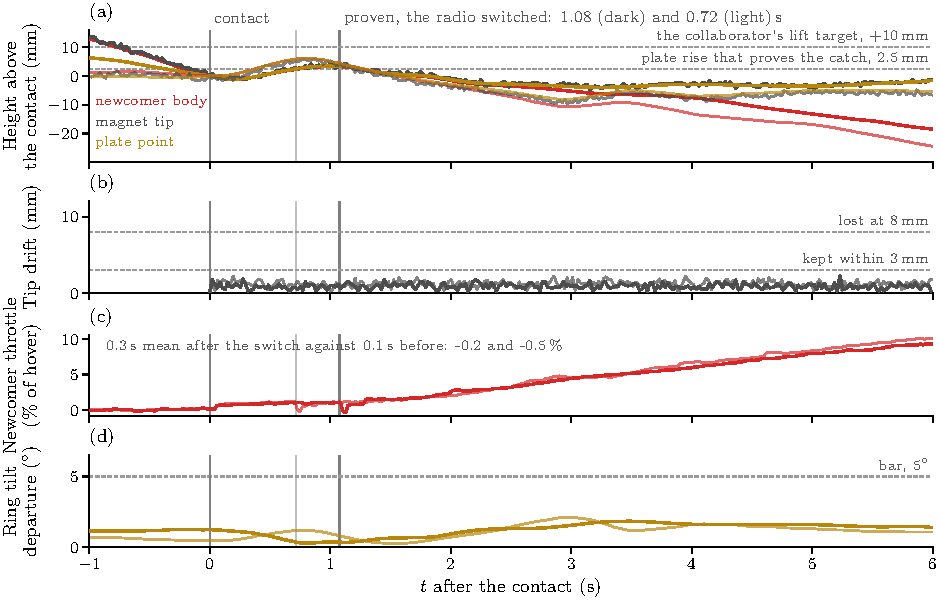
\includegraphics[width=\textwidth]{Images/proof_timeline.pdf}
\caption[The contact-and-lift proof]{The contact-and-lift proof in the twin: a newcomer flown by the collaborator's
controller comes down onto the plate at 90$^\circ$ of a hovering ring and the catch is proven from motion capture
alone. Two runs of the same arm, aligned on the contact: the darker run first, the lighter its repeat, which arrived
more slowly. (a) Heights above their value at the contact: the newcomer's body, its magnet tip (from the tip's own
marker, unfiltered) and the plate point (from the ring's pose). The collaborator's lift aims 10\,mm above the contact;
the catch is proven once the plate has risen 2.5\,mm with the tip and held it for 0.3\,s, which came 1.08 and
0.72\,s after the contact. (b) The tip's drift from the tip-to-plate vector it touched with, in the ring frame: a
proof needs it within 3\,mm and a contact is lost at 8\,mm. (c) The newcomer's throttle as a percentage of its hover
throttle: its radio switches to this work's tracker on the proof tick; the 0.3\,s mean after the switch differs from
the 0.1\,s before it by $-0.2$ and $-0.5$\,\%, and the rise that follows is the fold-in taking up its share of the
ring. (d) The ring's tilt departure from its mean over the 5\,s before the contact, against the 5$^\circ$ bar.}
\label{fig:F14}
\end{figure}

\begin{table}[htbp]
  \centering
  \footnotesize
  \caption{The twin claim (T11): the collaborator's controller flies the newcomer to contact and this work's proof
  admits it. Ranges over $n$ runs on one code tree. [Rows marked \emph{re-fly} come from the next tree's table.]}
  \label{tab:T11}
  \begin{tabularx}{\textwidth}{XcYYYYl}
    \toprule
    Claim line & $n$ & Contact to proof (s) & Throttle step (\%) & Ring tilt ($^\circ$) & Rod clearance (m)
      & Reviewer \\
    \midrule
    Attach, hover & 5 & 0.72--1.08 & 0.0--0.6 & 1.83--2.41 & $\ge 0.213$ & supported \\
    Attach, circle & 2 & 0.64--0.93 & 0.3--0.8 & 2.50--2.58 & [\dots] & with corrections \\
    Take-back, hover & 5 & -- & -- & 1.66--2.50 & $\ge 0.221$ & supported \\
    No catch, hover & 2 & -- & -- & [\dots] & [\dots] & supported \\
    LAND during the proof & 1 & -- & -- & [\dots] & [\dots] & supported \\
    Take-back, circle & [\dots] & -- & -- & [\dots] & [\dots] & \emph{re-fly} \\
    Push abort & [\dots] & [\dots] & [\dots] & [\dots] & [\dots] & \emph{re-fly} \\
    \bottomrule
  \end{tabularx}
\end{table}
% Hover attach also: proof to switch 0.000-0.003 s, newcomer tilt at the proof 0.04-0.32 deg, dip -0.4 to 1.6 mm,
% closest body 0.43-0.45 m. Hover take-back: attitude step 0.04-3.45 deg (3.45 in a LAND during his transit, between
% the 2 and 5 deg bars), down 17.4-18.8 s after the take-back. The table must not say: every circle take-back bar
% confirms; contact within 10 s (2 of 9); the hand-over attitude and yaw bars are confirmed (only the throttle step
% is scored). Report the first-contact timeouts (TB15).

\paragraph{Counterfactuals.} [Seed, force proof, hand-over step against TRADY's blend, the take-back.]

\paragraph{The proof on rig noise.} [The proof logic replayed over the rig bags and the 14 October hand catches:
false accepts and rejects, and the rig thresholds set from them. The twin's proof (1\,cm, rigid link) and the rig's
(slack tether, plate rise) are different protocols, and are stated as such.]

\pendingfig{fig:F15}{The first attaches on the rig: the no-catch flight, then the contact attach twice. [Caption.]}{The
14 October flights (sheet R6--R8); script on branch thesis-figs.}

\paragraph{Fault coverage and authority.} [One paragraph per tree. Twin, rig candidate tree: a tilt fault on the
newcomer while the collaborator flies it is caught 0.23--0.25\,s after the injected upset and the newcomer is
disarmed within 0.022\,s of the cut; with the switch off the newcomer stays armed (2 of 2); the freed UAV disarmed
alone [17 of 17]. Rig: no false cut over the rig bags [count from the offline sweep]; drop-on-loss armed on four rig
detaches with no false trigger. The matrix in an appendix.]
% Tilt card rev 4 on rig-wed ba40bd0: T1 R1662-R1663, C1 R1668-R1669, N1-N3 R1676-R1678 (fault 0.234-0.250 s after the
% injection; cut to disarm 0.003-0.022 s); T0 R1660-R1661. The reviewer scored T1 1 of 2 (the take-back race, fixed
% on week5 29b2d7b) and F1 1 of 2 (R1673, a true tumble in his flight).

\begin{table}[htbp]
  \centering
  \footnotesize
  \caption{The full mission (T12): the newcomer is released, picks up and drops the object with the collaborator's
  controller, and rejoins. [To fill from metrics.json, two hover and two circle runs under the full mission's card.]}
  \label{tab:T12}
  \begin{tabularx}{\textwidth}{lcYYYY}
    \toprule
    Path & $n$ & Release tilt ($^\circ$) & Reattached & Contact to proof (s) & Ring tilt at the attach ($^\circ$) \\
    \midrule
    Hover & [\dots] & [\dots] & [\dots] & [\dots] & [\dots] \\
    Circle & [\dots] & [\dots] & [\dots] & [\dots] & [\dots] \\
    \bottomrule
  \end{tabularx}
\end{table}
% Twin so far (exploratory, not under a card): hover end to end R1655; circle reattached in 6 of 7
% (R1523 R1541 R1564 R1579 R1631 R1633; R1656 missed: his ATTACH_READY lost alignment twice, then gave up). Reconcile
% R1523's 1.22 against 4.78 deg (plan 4.3.7).

\paragraph{Answer to RQ3.} [A quarter page.]
